Գրաֆների դեկարտյան արտադրյալների միջակայքային ներկումները առաջին անգամ դիտարկել են Գիառոն և Կուբալը 1997թ. \cite{GiaroKubale1997}: Մասնավորապես, հեղինակները ստացել էին որոշ արդյունքներ ցանցային տիպի գրաֆների վերաբերյալ: Առաջին ընդհանուր բնույթի արդյունքը ևս ստացել են նույն հեղինակները \cite{GiaroKubale2004,Kubale2004}.

\begin{theorem}
\label{t2_cartesian} Եթե $G,H\in \mathfrak{N}$, ապա $G\square H\in \mathfrak{N}$. Ընդ որում,
\begin{center}
$w(G\square H)\leq w(G)+w(H)$ և $W(G\square H)\geq W(G)+W(H)$:
\end{center}
\end{theorem}

Պետրոսյանը \cite{Petrosyan2011} ցույց է տվել, որ համասեռ գրաֆների դեպքում միայն մի արտադրիչի միջակայքային ներկելիությունը բավարար է արտադրյալի միջակայքային ներկելիության համար.
\begin{theorem}
\label{t2_kotzig} Եթե $G$ և $H$ գրաֆները համասեռ են և տեղի ունի հետևյալ պայմաններից գոնե մեկը.
\begin{enumerate}
\item $G$-ն և $H$-ը ունեն կատարյալ զուգակցում,
\item $G\in \mathfrak{N}$,
\item $H\in \mathfrak{N}$,
\end{enumerate}
ապա $G \square H \in \mathfrak{N}$:
\end{theorem}

Մենք ցույց կտանք, որ ոչ համասեռ գրաֆների դեպքում այս պնդումը միշտ չէ, որ տեղի ունի: Նախ նկատենք հետևյալ փաստը.

\begin{lemma}
\label{l2-cartesian-eulerian}
Եթե $G$-ն էյլերյան գրաֆ է, ունի զույգ թվով կողեր և կենտ թվով գագաթներ, իսկ $H$-ը կենտ թվով կողեր ունեցող էյլերյան գրաֆ է, ապա $G \square H$ արտադրյալը ևս էյլերյան է և ունի կենտ թվով կողեր:
\end{lemma}
\begin{proof}[Ապացույց]
$G\square H$ գրաֆը ակնհայտորեն էյլերյան է: Իսկ արտադրյալի կողերի քանակը՝ $|E(G \square H)| = |E(H)||V(G)| + |E(G)||V(H)|$, կենտ է, քանի որ $|E(G)|$-ն զույգ է, իսկ $|E(H)|$-ը և $|V(G)|$-ն՝ կենտ:
\end{proof}

Եթե վերցնենք կամայական էյլերյան գրաֆի երկու օրինակ և մի օրինակի որևէ գագաթ նույնացնենք մյուս օրինակի որևէ գագաթի հետ, ապա ստացված գրաֆը կարելի է վերցնել որպես լեմմայի $G$ գրաֆ: Մասնավորապես, այսպիսի գրաֆի օրինակ է թիթեռ գրաֆը, որն ունի միջակայքային ներկում (Աղ. \ref{table2-cartesian}): Որպես լեմմայի $H$ գրաֆ կարելի է վերցնել օրինակ $K_3$ եռանկյունը, որը միջակայքային ներկելի չէ: Այսպիսով թիթեռ գրաֆի և եռանկյան դեկարտյան արտադրյալը, ըստ Լեմմա \ref{l2-cartesian-eulerian}-ի, էյլերյան է և ունի կենտ թվով կողեր, ուստի, ըստ Հետևանք \ref{c1_eulerian}-ի, չունի միջակայքային ներկում:

Երկու միջակայքային չներկվող գրաֆների դեկարտյան արտադրյալը կարող է լինել ինչպես միջակայքային ներկելի, այնպես էլ չներկվող: Մասնավորապես, $P_{10}$ Պետերսենի գրաֆը չի բավարարում Թեորեմ \ref{t1_class1}-ի պայմանին, ուստի միջակայքային ներկելի չէ, սակայն երկու այդպիսի գրաֆների արտադրյալը $P_{10} \square P_{10}$ ներկելի է ըստ Թեորեմ \ref{t2_kotzig}-ի առաջին կետի: Մյուս կողմից, $C_{2n+1}$ կենտ երկարության ցիկլը, ինչպես նաև երկու այդպիսի ցիկլերի արտադրյալը չեն բավարարում Թեորեմ \ref{t1_class1}-ի պայմանին, ուստի չեն կարող ունենալ միջակայքային ներկում:

\begin{table}[h]
    \centering
    \begin{tabular}{c|c|c}
         & $G \square H \in \mathfrak{N}$ & $G \square H \notin \mathfrak{N}$ \\
         \hline
        $G \in \mathfrak{N}$, $H \in \mathfrak{N}$ & $G=H=K_2$ & հնարավոր չէ \\
        $G \in \mathfrak{N}$, $H \notin \mathfrak{N}$ & $G=K_2$, $H=K_3$ & $G=$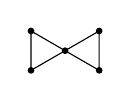
\begin{tikzpicture}[baseline=-0.5ex]
        \draw[fill=black] (0:0) circle(1pt);
        \draw[fill=black] (30:0.5cm) circle(1pt);
        \draw[fill=black] (-30:0.5cm) circle(1pt);
        \draw[fill=black] (150:0.5cm) circle(1pt);
        \draw[fill=black] (-150:0.5cm) circle(1pt);
        \draw (30:0.5cm) -- (0:0) -- (150:0.5cm) -- (-150:0.5cm) -- (0:0) -- (-30:0.5cm) -- cycle;
        \end{tikzpicture}, $H=K_3$ \\ 
        $G \notin \mathfrak{N}$, $H \notin \mathfrak{N}$ & $G=H=P_{10}$ & $G=H=K_3$ \\ 
        
    \end{tabular}
    \caption{Գրաֆների դեկարտյան արտադրյալների միջակայքային ներկելիության հարաբերությունը առանձին բաղադրիչների միջակայքային ներկելիության հետ՝ օրինակներով:}
    \label{table2-cartesian}
\end{table}

